%% 
%% Copyright 2007-2020 Elsevier Ltd
%% 
%% This file is part of the 'Elsarticle Bundle'.
%% ---------------------------------------------
%% 
%% It may be distributed under the conditions of the LaTeX Project Public
%% License, either version 1.2 of this license or (at your option) any
%% later version. The latest version of this license is in
%%    http://www.latex-project.org/lppl.txt
%% and version 1.2 or later is part of all distributions of LaTeX
%% version 1999/12/01 or later.
%% 
%% The list of all files belonging to the 'Elsarticle Bundle' is
%% given in the file `manifest.txt'.
%% 
%% Template article for Elsevier's document class `elsarticle'
%% with harvard style bibliographic references

\documentclass[preprint,12pt,authoryear]{elsarticle}

%% Use the option review to obtain double line spacing
%% \documentclass[authoryear,preprint,review,12pt]{elsarticle}

%% Use the options 1p,twocolumn; 3p; 3p,twocolumn; 5p; or 5p,twocolumn
%% for a journal layout:
%% \documentclass[final,1p,times,authoryear]{elsarticle}
%% \documentclass[final,1p,times,twocolumn,authoryear]{elsarticle}
%% \documentclass[final,3p,times,authoryear]{elsarticle}
%% \documentclass[final,3p,times,twocolumn,authoryear]{elsarticle}
%% \documentclass[final,5p,times,authoryear]{elsarticle}
%% \documentclass[final,5p,times,twocolumn,authoryear]{elsarticle}

%% For including figures, graphicx.sty has been loaded in
%% elsarticle.cls. If you prefer to use the old commands
%% please give \usepackage{epsfig}

%% The amssymb package provides various useful mathematical symbols
\usepackage{amssymb}
%% The amsthm package provides extended theorem environments
%% \usepackage{amsthm}

%% The lineno packages adds line numbers. Start line numbering with
%% \begin{linenumbers}, end it with \end{linenumbers}. Or switch it on
%% for the whole article with \linenumbers.
%% \usepackage{lineno}

\journal{Poetics}

\begin{document}

\begin{frontmatter}

%% Title, authors and addresses

%% use the tnoteref command within \title for footnotes;
%% use the tnotetext command for theassociated footnote;
%% use the fnref command within \author or \affiliation for footnotes;
%% use the fntext command for theassociated footnote;
%% use the corref command within \author for corresponding author footnotes;
%% use the cortext command for theassociated footnote;
%% use the ead command for the email address,
%% and the form \ead[url] for the home page:
%% \title{Title\tnoteref{label1}}
%% \tnotetext[label1]{}
%% \author{Name\corref{cor1}\fnref{label2}}
%% \ead{email address}
%% \ead[url]{home page}
%% \fntext[label2]{}
%% \cortext[cor1]{}
%% \affiliation{organization={},
%%            addressline={}, 
%%            city={},
%%            postcode={}, 
%%            state={},
%%            country={}}
%% \fntext[label3]{}

\title{Aligning Our Toolkits With Our Intuitions: Local Structural Models of Cultural Networks}

%% use optional labels to link authors explicitly to addresses:
%% \author[label1,label2]{}
%% \affiliation[label1]{organization={},
%%             addressline={},
%%             city={},
%%             postcode={},
%%             state={},
%%             country={}}
%%
%% \affiliation[label2]{organization={},
%%             addressline={},
%%             city={},
%%             postcode={},
%%             state={},
%%             country={}}

\author[inst1]{Omar Lizardo}

\affiliation[inst1]{organization={University of California, Los Angeles},%Department and Organization
            addressline={264 Haines Hall}, 
            city={Los Angeles},
            postcode={90095}, 
            state={CA},
            country={USA}}


\begin{abstract}
%% Text of abstract

\end{abstract}

%%Graphical abstract
%\begin{graphicalabstract}
%\includegraphics{grabs}
%\end{graphicalabstract}

%%Research highlights
\begin{highlights}
\item Research highlight 1
\item Research highlight 2
\end{highlights}

\begin{keyword}
%% keywords here, in the form: keyword \sep keyword
Cultural Networks \sep Local Structure \sep Neighborhoods \sep Exponential Random Graph Models
%% PACS codes here, in the form: \PACS code \sep code
%\PACS 0000 \sep 1111
%% MSC codes here, in the form: \MSC code \sep code
%% or \MSC[2008] code \sep code (2000 is the default)
%\MSC 0000 \sep 1111
\end{keyword}

\end{frontmatter}

%% \linenumbers

%% main text
\section{Introduction}
\label{sec:intro}
Recent years have seen a resurgence of work in cultural sociology that incorporates substantive and methodological ideas from network analysis to address core issues in studying taste, cultural consumption, and the structure and dynamics of ``cultural networks" more generally.

Despite this efflorescence of work---and perhaps very much because of it---we stand at a curious impasse in studying taste and cultural consumption. The problem is this: While the core intuitions of the field are becoming increasingly ``formalist'' and ``relationalist,''\footnote{See \citet{erikson2013formalist} for the distinction between formalist and relationism in social network analysis. The distinction is undoubtedly important but not crucial for my broad argument. Therefore, in what follows, I will use ``formalist,'' ``formalism'', ``relational,'' and ``relationalist'' interchangeably to refer to the cluster of intuitions that come packaged with network analytic thinking and which have been increasingly used to understand cultural tastes and cultural networks.} the core workhorse methods in the field, such as traditional regression analysis (and its various non-linear and mixed effects variations), latent class analysis, various data reduction techniques like factor and cluster analysis, and the now widely used geometric data analytic techniques only cash in those formalist intuitions in either very indirect or roundabout ways. 

Meanwhile, the recently introduced suite of network-inspired techniques, while useful for recasting core notions in a more relational mold, lacks the natural unity and compatibility with thinking of the world as governed by chance, uncertainty, and probability as statistically grounded techniques like the general linear model or latent class analysis. 

In this paper, I argue that a general, statistically and probabilistically grounded approach to thinking about how the local structuration of network ties gives rise to macro-structural patterns tied to a now relatively accessible, well-developed and mature framework for the statistical analysis of network structures---typically going by the offputting and unwieldy name of ``exponential random graph models,'' can serve to align the increasingly formalist intuitions quantitatively inspired cultural analysis bring to the study of tastes and culture consumption, with a coherent methodological approach that cashes in those intuitions \textit{directly}, while at the same time incorporating into a schema that is familiar to those whose go-to is the typical regression model. 

The rest of the paper is organized as follows. in section~\ref{sec:networks}, I briefly review recent formalist work incorporating network ideas into the sociology of taste, concentrating on its conceptual and measurement accomplishments but also its limitations. In section~\ref{sec:localstruct}, I outline the \textit{intuition/method gap} separating our increasingly formalist ideas about how cultural networks work from the traditional analytic toolkit. In section~\ref{sec:data}, I introduce the data to be analyzed---a standard survey of the musical tastes of a representative sample of Americans---and in~\ref{sec:ermgs}, I provide a brief introduction to the local structural framework of exponential random graph models for two-mode networks \citep{pattison2002neighborhood}, which promises to close the aforementioned intuition/method gap by providing estimates and insight into all the local structural intuitions in a single mode. In section~\ref{sec:disc}, I close by outlining the implications of the results and the larger argument for future work in the sociology of taste. 

\section{The Rise of Network Thinking in the Sociology of Taste}
\label{sec:networks}

\section{Three Relational Intuitions versus the Standard Methods}
\label{sec:localstruct}

In this section, I revisit a series of ``formalist" intuitions sociologists of taste have about core phenomena in the field and review how the usual methods would handle them. At the end of the section, I propose that probabilistic network analysis focused on local structures provides a more elegant and unified way of considering them and providing an opportunity to even pit them against one another. 

\subsection{Breadth of Taste and Popularity}
I begin with the simplest relationist notion in the sociology of taste, which concerns the idea that people---and, by implication, groups---differ in the \textit{breadth} or \textit{extensiveness} of their tastes. In a cultural network, for the people, this would yield the notion of \textit{degree centrality}, which translated into the conceptual apparatus of the sociology of taste matches the notion of \textit{omnivorousness by volume} (OV) proposed by \citet{warde2009anatomy}---see \citet{lizardo2014omnivorousness} for further discussion. 

The usual toolkit of methods can be used to analyze group differences in OV in various ways. For instance, we could specify OV as the outcome variable in a linear or count regression model. Then, we can look at coefficient estimates of various socio-demographic predictors to ascertain group differences in the number of genres or objects chosen. The usual linear regression-based methods are useful for codifying group differences in average OV but lose track of the underlying micro-structures that generate these differences at the level of local neighborhoods. These are shown in Figure~\ref{fig:local-struct1}(a). 

The diagram uses circles to represent individuals and squares to represent cultural objects, with lines showing the connections between people and objects. Shaded circles and squares indicate differences in characteristics. Unshaded circles and squares (those filled in white) are considered "unmarked," implying generalization across all their traits. The research on group differences in OV revolves around variations in connectivity in the cultural network among individuals from different groups. Some types of individuals are shown to connect to only a few objects (lighter shade of gray circle), while others connect to many objects (darker shade of gray circle).

One advantage of using local structural specification is that it allows us to easily change perspectives and examine cultural objects in the same way. As depicted in Figure~\ref{fig:local-struct1}(b), variations in the breadth or audience reach of objects result in differences in their \textit{popularity}, distinguishing popular objects with wide audiences from niche objects with smaller audiences \citep{lizardo2018mutual}. From the viewpoint of the cultural network, these differences simply represent variations in the objects' centrality in the other mode \citep{faust1997centrality}. These ideas are already evident in many standard approaches, such as using techniques like factor or principal components analysis to categorize cultural sets of genres or objects into ``pop" and "niche" clusters (e.g., ``highbrow," ``folk").

It is challenging to incorporate factors related to differences in the audience reach of various types of objects into our standard models. In a recent study, \citet{puetz2021taste} creatively combined information about differences in the popularity of objects chosen by people with differences in consumption style among individuals, using these as outcome variables in linear regression. This meant shifting the focus of analysis from objects to people, as linear regression typically deals with one unit of analysis at a time. However, the \textit{simultaneous} consideration of differences in breadth and popularity between people and objects within the same modeling framework, as required by our formalist intuitions, cannot be accommodated by traditional strategies. As we will see, these considerations can be easily dealt with in the proposed local structural framework.

\subsection{Correlated choices for people and objects}
The need for a more flexible framework becomes evident once we consider local relational intuitions of greater complexity than those related to breadth and popularity. Consider the standard---sometimes explicit but usually implicit---justification for clumping people and cultural objects into ``kinds'' in the first place (e.g., sociodemographic groups on paper or genre clusters). 

I propose that the local-structural relational intuition that such clustering is grounded on is as presented in Figure~\ref{fig:local-struct2}(a) and (b). The basic justification for using data-reduction techniques, such as cluster or factor analysis, to clump cultural objects is that we presume that there is a local structural affinity between the objects under the clump, such that they tend to be chosen together by the same people. For instance, ``highbrow'' musical genres like Opera, Jazz, and Classical will tend to be chosen together, as are ``Folk'' genres like Country and Bluegrass. In terms of local structural configurations, this implies a substantive restriction in the types of ``two-paths'' we will tend to observe in the cultural networks, such that two paths featuring two objects in the same broad category joined by a person who chooses them both will be more likely to be observed than two-paths were the objects belong to different genre clusters, as shown in Figure~\ref{fig:local-struct2}(a).\footnote{In a cultural (two-mode) network, a ``two-path'' is any contiguous sequence of three nodes (a, B, c) and two edges (a---B and B---c), with two of the nodes (in this case, a and c) necessarily belonging to one mode and the other (in this case B) to the other mode, as links can only happen between nodes in different modes. In a cultural network, two paths can result from any person (B) choosing any two objects (a, c) or any two people (a, c) choosing the same object (B).} 

Dually, although not usually expressed in these terms, socio-demographic similarities between people imply, at the local structural level, commonality in cultural choices. This is, in fact, the local structural consideration given for why we should observe cultural objects occupying distinct ``niches'' in sociodemographic space---provided that patterns of association between people are socially structured such that similar people are more likely to be connected \citep{mark2003culture, dellaposta2015liberals}. This is the local structural pattern shown in Figure~\ref{fig:local-struct2}(b).

Traditional methods can no doubt be mobilized to explore these possibilities, especially those concerned with sociodemographic effects on common cultural choices. For instance, given a battery of cultural items, we can compute regression models with these items as outcomes and check to see which coefficient estimates show up with the same direction and patterns of statistical significance across models, indicating that people in those groups tend to choose (or abstain from) those items. In the same way, we could use standard geometric data analysis (GDA) techniques for multivariate data \citep{le2004geometric}, like Multiple Correspondence Analysis (MCA), to construct a ``social space'' composed of the different cultural items with proximities indicating the likelihood of being chosen together and then ``project'' socio-demographic categories into the space---by computing the average values of the various socio-demographic modalities across the relevant axes---to see which groups are doing the common choosing \citep{flemmen2018social, le2008class}.\footnote{This can also be done the other way around, constructing a social space of active demographic variables and projecting choices into the space; the result is the same intuition: People belonging to the same groups on paper make common cultural choices.} 

The GDA approach is definitely much less awkward and more direct than the endless series of regression models approach and, thus, closer to the relational intuitions- not a surprise, given the relational bona fides of GDA. Yet, GDA remains a \textit{global} relational strategy, forcing the analyst, in the end, to rely on average approximations of the relevant local structural patterns rather than modeling those directly. 

\subsection{Social closure in cultural choices}

\section{Data}
\label{sec:data}
\section{Exponential Random Graph Models for Two-Mode Networks}
\label{sec:ermgs}
\section{Results}
\label{sec:results}
\section{Discussion and Conclusion}
\label{sec:disc}


%% For citations use: 
%%       \citet{<label>} ==> Jones et al. (2015)
%%       \citep{<label>} ==> (Jones et al., 2015)



%% The Appendices part is started with the command \appendix;
%% appendix sections are then done as normal sections

%% If you have bibdatabase file and want bibtex to generate the
%% bibitems, please use
%%
\newpage
\bibliographystyle{elsarticle-harv} 
\bibliography{refs}

%% else use the following coding to input the bibitems directly in the
%% TeX file.

% \begin{thebibliography}{00}

% %% \bibitem[Author(year)]{label}
% %% Text of bibliographic item

% \bibitem[ ()]{}

% \end{thebibliography}

\begin{figure}
    \centering
    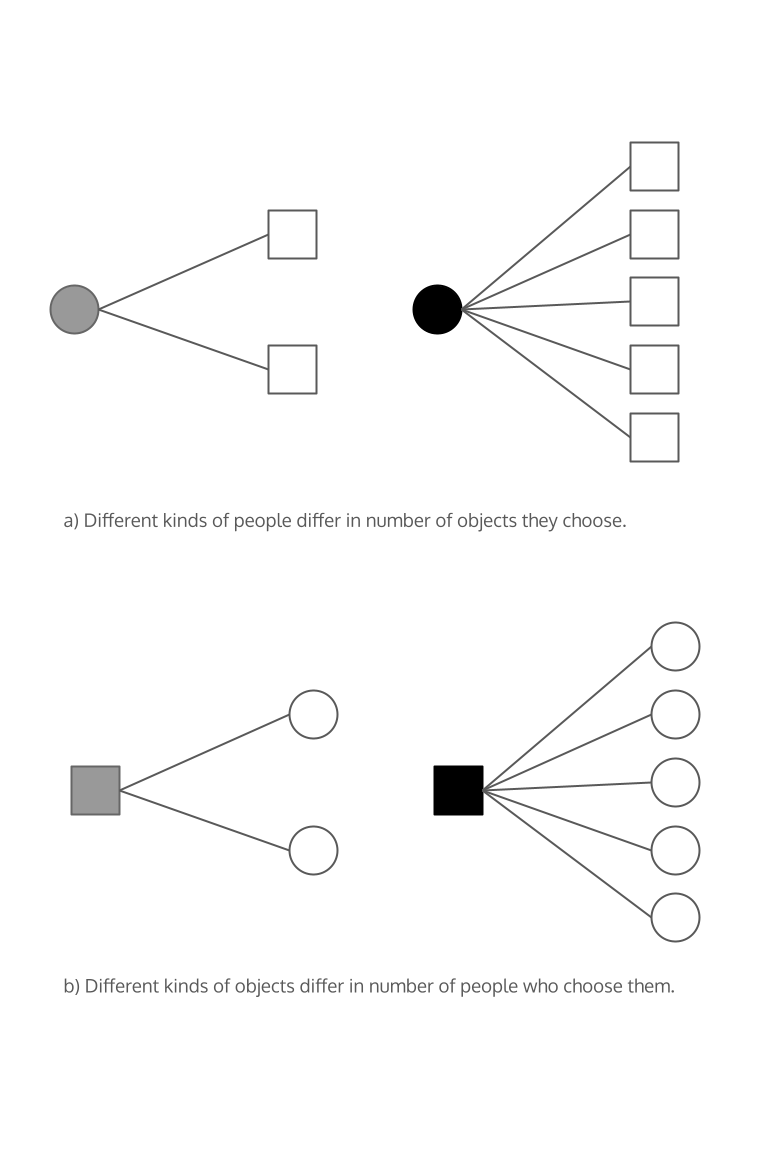
\includegraphics[width=0.8\linewidth]{Figs/local-struct1.png}
    \caption{Local structural neighborhoods of omnivorousness and popularity}
    \label{fig:local-struct1}
\end{figure}

\newpage

\begin{figure}
    \centering
    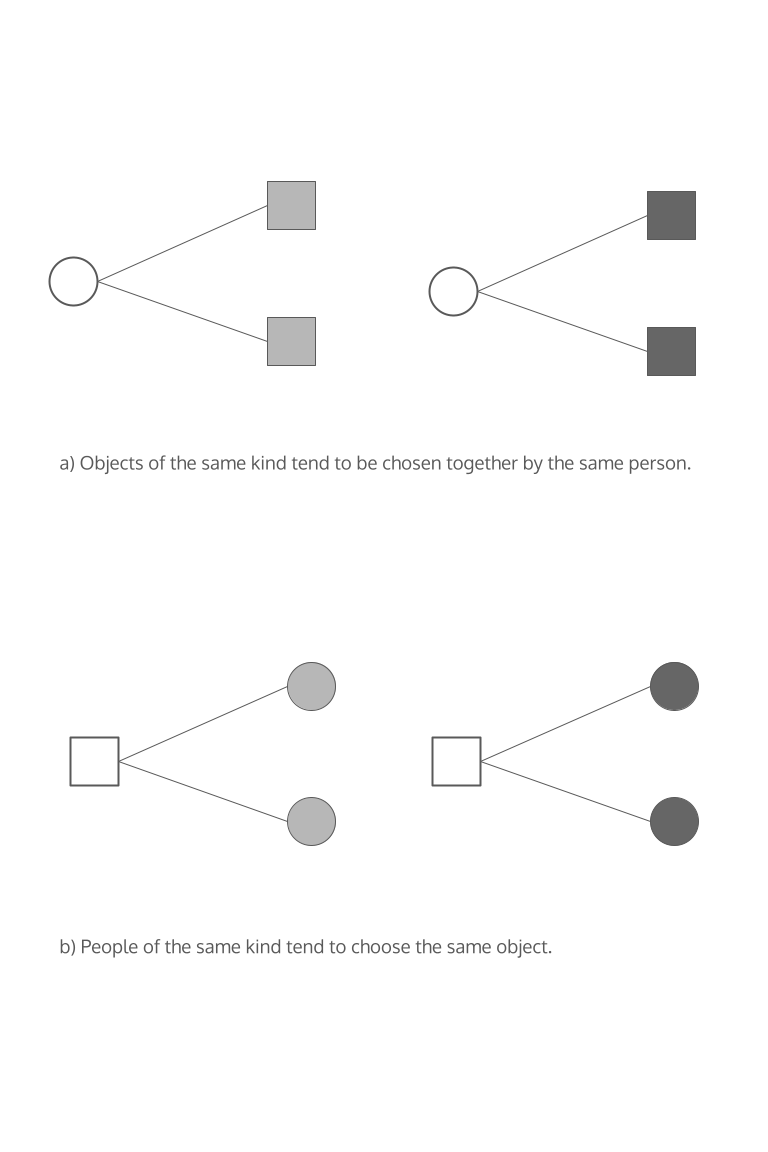
\includegraphics[width=0.8\linewidth]{Figs/local-struct2.png}
    \caption{Local structural neighborhoods of correlated choices}
    \label{fig:local-struct2}
\end{figure}

\end{document}

\endinput
%%
%% End of file `elsarticle-template-harv.tex'.
